\subsubsection*{5. Bestem den maksimale værdi af Vout i de to tilfælde.}

For at finde den maksimale værdi af $V_{out}$ for de 2 grafer, kan det ved 1 k$\Omega$ måles ud fra grafen, mens det ved 10 k$\Omega$ både kan beregnes og måles.

$V_{max}$ for 1 k$\Omega$ = 5.766, som det også kan ses på nedstående graf. 

\begin{figure}[h]
 \begin{center}
  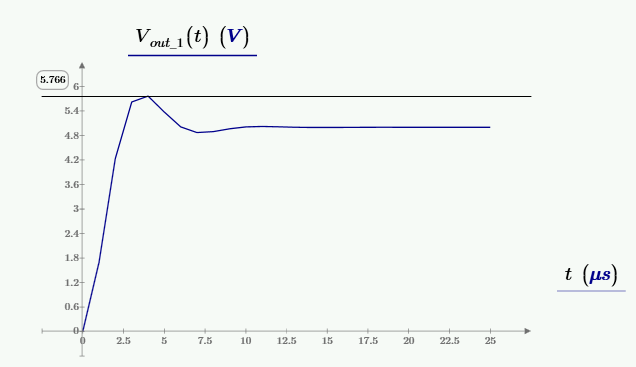
\includegraphics[height=5cm]{P_Fig/figur16_ana2graf1Kmax}
  \caption{$V_{max} 1 k\Omega$}
  \label{max1K}
 \end{center}
\end{figure}

Ved 10 k$\Omega$, kan dette beregnes ved at sætte tiden t til 100 procent i dette tilfælde vil det sige 100 $\mu s$

\begin{equation}
V_{max\_10} = V_{out\_10}(100\mu s)  = 5 V
\end{equation} 

Dette kan også ses på nedenstående graf:

\begin{figure}[h]
 \begin{center}
  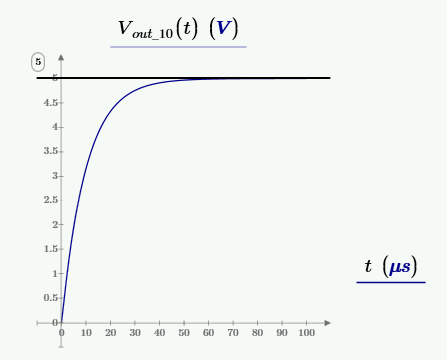
\includegraphics[height=5cm]{P_Fig/figur17_ana2graf10Kmax}
  \caption{$V_{max}$ 10 k$\Omega$}
  \label{max10K}
 \end{center}
\end{figure}